\documentclass[11pt]{article}

\usepackage[margin=1in]{geometry}
\setlength{\headheight}{13.6pt}
\usepackage{fancyhdr}
\pagestyle{fancy}
\usepackage{scalerel}
\usepackage{mathtools}
\usepackage{amssymb}
\usepackage{xparse}
\usepackage{csquotes}
\usepackage{float}
\usepackage[inline]{enumitem}
\usepackage[htt]{hyphenat}
\usepackage{circuitikz}
\usepackage{siunitx}
\usepackage{tikz}
\usetikzlibrary{arrows}
\usetikzlibrary{arrows.meta,quotes}
\usetikzlibrary{automata,positioning}

% Makes \setItemLetter work
\ExplSyntaxOn
\DeclareExpandableDocumentCommand \AlphToNum { m }
{
   \int_from_alph:n { #1 }
}
\ExplSyntaxOff

\makeatletter
% Changes the number on an \item
\newcommand\setItemNumber[1]{\setcounter{enumi}{\numexpr#1-1\relax}}
% Changes the letter on an \item
\newcommand\setItemLetter[1]{\setcounter{enum\romannumeral\enit@depth}{\numexpr\AlphToNum{#1}-1}}
\makeatother
% Aligns the top of a displaymath environment with the top of an \item
\newcommand\DisplayMathItem[1][]{%
  \ifx\relax#1\relax  \item \else \item[#1] \fi
  \abovedisplayskip=0pt\abovedisplayshortskip=0pt~\vspace*{-\baselineskip}}

%\setlength{\parindent}{0em}

\lhead{Final Project Design}
\chead{Jason Chen --- Travis Whitehead}
\rhead{June 12, 2019}

\begin{document}

\noindent
{\huge\textbf{Architecture Diagram}}\bigskip

A diagram of our API's architecture is in Figure \ref{fig:architecture}.

\begin{figure}[H]
  \centering
  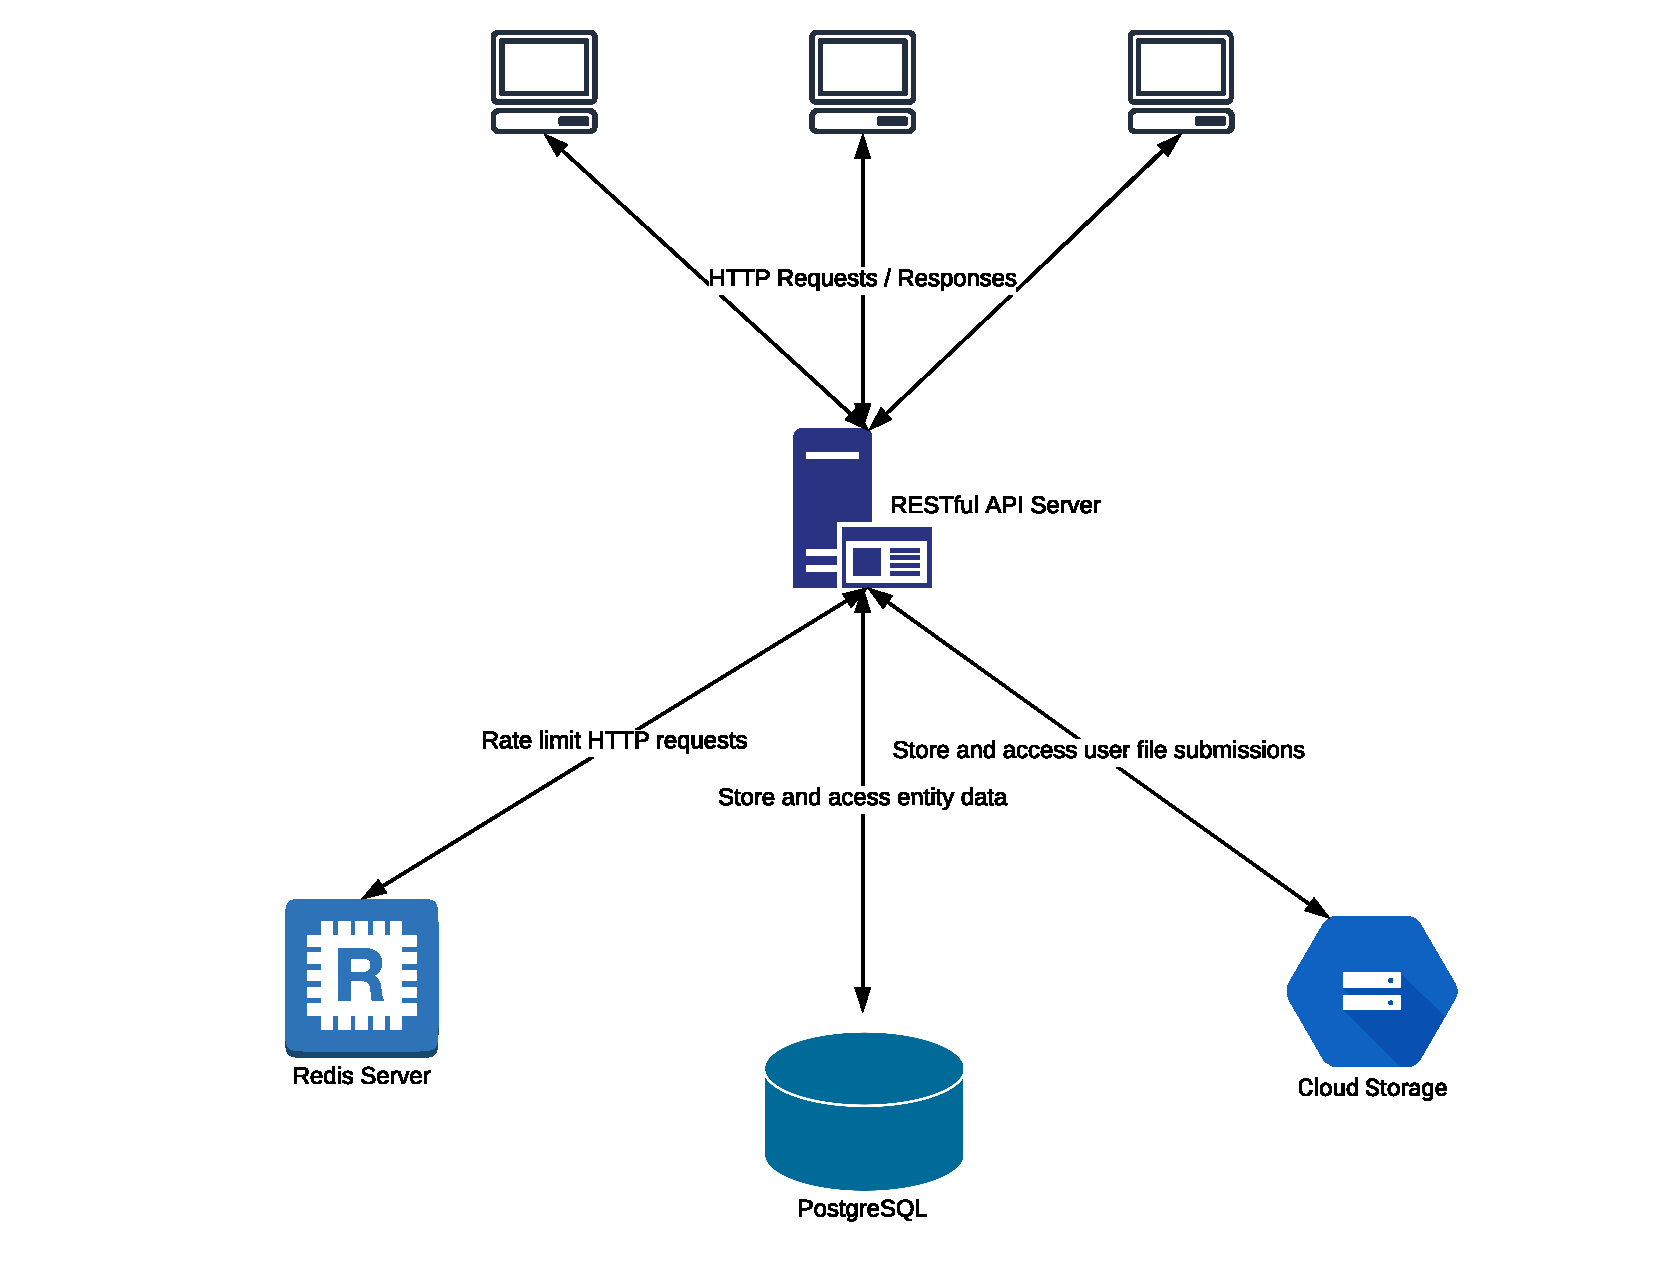
\includegraphics[width=.70\linewidth]{./architecture.pdf}
  \caption{Diagram of the high-level architecture of our final project. The API server uses Redis to rate limit incoming HTTP requests. All data, with the exception of student file submissions, is stored in a relational PostgreSQL database. Student file submissions are stored separately in a Google Cloud Storage bucket.}
  \label{fig:architecture}
\end{figure}

\bigskip
\bigskip

\noindent
{\huge\textbf{Data Layout}}\bigskip

Our database has five tables: \texttt{users}, \texttt{courses}, \texttt{assignments}, \texttt{course\_students}, and \texttt{assignment\_submissions}. The \texttt{users} table has columns for name, email address, password, and the user's role. A user has a single role and must be an administrator, an instructor, or a student. Each user's email must be unique, so no two user rows can be associated with the same email address.

The \texttt{courses} table contains columns for subject, course number, title, term, and the user ID of the course's instructor. The instructor's user ID is a foreign key on the \texttt{courses} table, representing the many-to-one relationship between \texttt{courses} and instructors. In other words, many courses may be taught by the same instructor, and one instructor may teach multiple courses.

The \texttt{assignments} table has columns for title, number of points, due date, and the ID of the course to which an assignment is associated. The due date is a timestamp in the requested format. The course ID foreign key indicates the many-to-one relationship between \texttt{assignments} and \texttt{courses}. Many assignments can be given in the same course, and one course can have many assignments.

The \texttt{course\_students} table has columns for a course ID and a student ID. The purpose of this table is to represent the many-to-many relationship between \texttt{courses} and \texttt{students}. A course can have many students enrolled, and a student may enroll in many courses. This table keeps track of enrollments by linking the \texttt{courses} and \texttt{students} tables.

Finally, the \texttt{assignment\_submissions} table stores student-uploaded submissions of assignments. It contains columns for assignment ID, student ID, enrollment ID, a timestamp of when the submission occurred, the original filename of the submission, and the name of the file stored in Google Cloud Storage. The assignment and student ID fields associate the submission with a specific assignment and student (many-to-one relationships). The enrollment ID is a foreign key that references the \texttt{course\_students} table. The purpose is to properly delete submissions when a student unenrolls from a course or a course is deleted. Additionally, student-uploaded files are stored in Google Cloud Storage, so the table also keeps track of a submission's filename inside the storage bucket, allowing for easy file retrieval.

Separate from the relational data, the API server also uses a Redis datastore to perform IP-based rate limiting. At the beginning of every request, the server increments a key associated with the client's IP and the current minute. If the incremented value of that key is greater than the maximum number of allowed requests per minute, the request does not get processed, and an appropriate response is returned to the client.

\bigskip
\bigskip

\noindent
{\huge\textbf{Reflection}}\bigskip

We chose this particular architecture and data layout based on our familiarity with the technologies used. Both of our team members have worked with PostgreSQL (and relational databases in general) more extensively than MongoDB, so we decided to use a relational database. Using PostgreSQL also made sense because the data entities---courses, users, assignments---are all related in ways that can be represented efficiently and easily using a relational database. For example, courses have many students; students can belong to many courses; assignments are associated with only one course. Those are all things that are naturally modeled as relational data.

In addition to the four tables representing those entities and assignment submissions, we chose to create a fifth table that links courses and students. Because students can be a part of many courses, and courses have many students, that relationship could not be represented in a sane way without an additional table. It also allows the deletion of a course or user to cascade to different tables. For example, if a student is deleted, their enrollment in a course should also be removed. The foreign key constraints in PostgreSQL allow that behavior very easily.

Along with PostgreSQL, we chose to use Redis to perform rate-limiting because it's a very fast in-memory store. Rate limiting does not require storing large amounts of data, so the quick lookup performance of Redis is a great way to keep track of and restrict the number of incoming requests without adversely affecting the API server's performance. Adding Redis as a simple rate-limiting tool now also allows flexibility in the future, when we may want to add a message queue, caching, or other behavior that requires storing and accessing data quickly.

Finally, we decided to use Google Cloud Storage (GCS) so we don't have to worry about storage requirements on the API server. GCS has a very simple and flexible API that can provide quick read-only access to files. When users request to download an assignment submission, we can simply give them a signed GCS URL that is accessible for a limited amount of time. Using GCS makes the application more scalable since the API server does not have to worry about serving large amounts of static data.

Overall, we are happy with the design of the program. Using Redis to rate-limit and GCS to serve files were both easy to implement and work very well. Storing all of the entity data in PostgreSQL also worked well, but the relational database libraries in Node.js can be awkward to work with. Unlike with MongoDB, which works naturally with JSON data, using the PostgreSQL library requires large amounts of raw SQL queries that end up becoming very reptitive.

So the biggest part of the program that we would change is to use an ORM library to work with the database, instead of writing raw queries and converting the results into JavaScript objects. Give the small scope of the application, using an ORM would have been appropriate for now.

\end{document}
